% \documentclass[linenumbers,summarypage,hyperlinks]{outhesis}
\documentclass{outhesis}

% For a bibliography style, you must have the appropriate .bst file
% \bibliographystyle{apj}
\bibliographystyle{prsty}

% Provide the correct margins
\usepackage[top=1in, bottom=1in, left=1.6in, right=1.2in]{geometry}
% If you want a double-sided copy for yourself, uncomment the next line
 % \usepackage[twoside,top=1in, bottom=1in, left=1.6in, right=1.2in]{geometry}

\begin{document}

%% Place Dissertation information here
%% Follow the convention for the use of capital letters 
%% or else the font will not be formatted properly
\author{Othmane Rifki}
\university{UNIVERSITY OF OKLAHOMA}
\college{GRADUATE COLLEGE}
\department{HOMER L. DODGE DEPARTMENT OF PHYSICS AND ASTRONOMY}
\title{THE MUON ANOMALOUS MAGNETIC MOMENT:\\ A PROBE FOR NEW PHYSICS}
\address{Norman, Oklahoma}
\yr{2014}
\dgname{SPECIALIST'S EXAMINATION}
%% List your committee members here
\committee{{Dr. Brad Abbott, Chair}, {Dr. S. Lakshmivarahan, Outside Member}, Dr. Mike Strauss, Dr. Chung Kao, Dr. Eric Abraham}

%% Put your dedication here. This is completely optional. Delete it if you don't need it.
%\begin{dedication}
 % 
%\end{dedication}

%% Put your acknowledgements here. This is completely optional. Delete it if you don't need it.
%\begin{acknowledgements}
%  
% \end{acknowledgements}

%% Put your abstract here.

\begin{abstract}
Every particle has an intrinsic magnetic moment due to its spin angular momentum characterized by a constant $g$, called the gyromagnetic ratio, that is very close to the value 2. The experimental measurement of this quantity to a very high accuracy has made it one of the most precisely measured quantities in particle physics. This measurement when compared with the theoretical predictions of the Standard Model of particle physics shows a difference in the order of 3 standard deviation which suggests the possibility of new physics. The goal of this review is to describe the measurements done in the past, and the improvements that the Fermilab $g-2$ experiment will achieve.

\end{abstract}


\frontmatter

\maketitle

\mainmatter



\section{Introduction}


The development in our understanding of the elements that form the physical world around us and the laws that govern it has been pursued through two complementary routes. On one hand, the empirical observation of phenomena led to mathematical formulations that describe them and predict their future. On the other hand, these mathematical models are also used to predict new phenomena not yet observed. In this sense, physics can be defined as a two way street where experiment (empirical observations) checks the theory (mathematical formulations), while the theory pave new ground for experiments. It is by going back and forth between these two approaches that we test the robustness of our understanding of the properties of our universe. For instance, the study of elementary particles and their interactions, the field of particle physics, has constructed a theoretical formulation, known as the \emph{Standard Model} (SM). When subjected to experimental tests, the SM successfully describes three of the four fundamental forces; electromagnetic, weak, and strong interactions. On the other hand, the SM is not believed to be complete since it does not incorporate the fourth fundamental force of gravity and it does not answer 
some fundamental problems that are facing today's physics community such as the nature of the ``invisible'' matter that is holding galaxies together which constitutes $\sim$ 26\% of the energy density of the universe, known as \emph{Dark Matter}, the different masses and mixing of the 12 leptons\footnote{Leptons are the electron neutrino and the electron, the muon neutrino and the muon, and the tau neutrino and the tau, in addition to their six anti-particles } knows as the \emph{flavor problem}, and the predominance of matter over antimatter. 
 
For these reasons and many others, searches of physics not incorporated in the SM has been underway in both theory and experiment. Any sign of significant discrepancy between theory and experiment is taken very seriously since it might lead to new insights that can reveal what is missing in our current view of the universe. While some experiments have looked for answers to these problems by studying high energy interactions as it is pursued at the Large Hadron Collider near Geneva, in the hope of observing some new particles - for instance the discovery of the Higgs boson in 2012, a central piece of the SM - others have performed detailed studies of known particles by measuring their properties to very high accuracies and comparing them to theoretical calculations to both check the models and look for discrepancies. The subject of this current review is an important illustration of the latter scenario where we examine precision tests of the intrinsic property of a spinning charged elementary particle known as the \emph{magnetic moment} by comparing theory to experiment.

The possible elementary charged particles that can be used to measure the magnetic moment are the three spin $\frac{1}{2}$ leptons: the electron $e$, the muon $\mu$, and the tau $\tau$. While these particles have the same charge and spin, they have very different masses which are given by $m_e$ = 0.511 MeV$/c^2$ \footnote{The unit of mass is given by MeV/c$^2$ according to the relation E = mc$^2$ with the energy E given in units of MeV where 1MeV = 1.6 $\times$ 10$^{-13}$J.}, $m_{\mu}$ = 105.658 MeV$/c^2$, and $m_{\tau}$ = 1776.99 MeV$/c^2$. The difference in masses alters the lifetimes and decay modes of each particle. The electron is the lowest mass charged lepton and thus is stable, the muon lifetime is $\tau_{\mu} = 2.197 \times 10^{-6}$ seconds and it decays almost 100\% to an election and two neutrinos ($e\nu_{\mu}\bar{\nu_{e}}$), while taus have a much shorter lifetime $\tau_{\tau} = 2.906 \times 10^{-13}$ seconds and a diversified decay pattern where 65\% go into hadronic states (states that contain quark-antiquark pair particles such as pions) and the remainder are leptonic decays to muons or electrons and two neutrinos. Because of its very short lifetime, the study of the tau's magnetic moment is not possible using our current technology, leaving the electron and the muon as the appropriate candidates. While the electron is the most precisely studied lepton, the effects in the magnetic moment that are sensitive to physics beyond the SM scale with powers of $m_\ell^2$ ($\ell$ refers to the lepton) [\textbf{ref?}]. For this reason, muons are more appropriate for the study of the magnetic moment to search for new physics. 
The origin of the magnetic moment arises from the electric charge and the current of an elementary charged particle with spin. For instance, a classical calculation (see Appendix \ref{app:bmt}) of a particle with mass m and charge q moving in a circular orbit of radius $r$ with velocity $\overrightarrow{v}$, shows that its magnetic moment ($\overrightarrow{\mu}$) is related to its orbital angular momentum ($\overrightarrow{L} =m\overrightarrow{r} \times \overrightarrow{v}$) by the relation:

\begin{equation}
\overrightarrow{\mu} = \frac{q}{2mc} \overrightarrow{L}
  \label{eq:L}
\end{equation}

In quantum mechanics, the magnetic moment is an \emph{intrinsic} property of a particle with spin. Both the magnetic moment and the orbital angular momentum are replaced by operators to give the correct quantum mechanical representation. While equation \ref{eq:L} is still valid for describing orbital angular momentum, spin magnetic moment requires a modification by a factor $g$ that is very close to 2. The corrected equation is given by

\begin{equation}
\overrightarrow{\mu} = g\frac{q}{2mc}\overrightarrow{S}
\label{eq:mu}
\end{equation}

where $g$ is called the \emph{gyromagnetic ratio} or \emph{g-factor}, and $q$ is the charge given in units of the fundamental charge $e$ where $q = -e$ for a lepton particle (negative muon) and $q = +e$ for a lepton anti-particle (positive muon). 

The result $g = 2$ was first obtained by Dirac when he generalized the Schroedinger equation to incorporate special relativity. With the development of the quantum mechanical description of electromagnetism known as quantum electrodynamics (QED), $g$ was found to differ from 2 by an anomaly $a_\ell$ ($\ell$ stands for a lepton), known as the  \emph{magnetic moment anomaly} such that: $g_\ell = 2(1+a_\ell)$. By solving for the anomaly $a_\ell$, the anomalous magnetic moment expression is obtained,

\begin{equation}
a_{\ell} = \frac{g_\ell-2}{2}
\end{equation}


The $g-2$ factor appeared! This is the title of all experiments that measure the magnetic moment of the muon and it is the focus of this review.

In addition to the quantum fluctuations of the electromagnetic field described by QED, the anomaly is also due to quantum fluctuations due to heavier particles such as the weak gauge bosons (W$^{\pm}$ and Z bosons) and hadrons (for example quark-antiquark pairs such as pions). These effects are known as radiative corrections (RC) and are mainly dominated by QED as it will be discussed in section \ref{sec:sm}.\\
In fact, the anomaly scales as $\delta a_\ell \sim \frac{m_\ell^2}{M^2}$  where M$\gg m_\ell$ can represent the mass of a heavier SM particle, the mass of an unobserved heavy particle beyond the SM, or an energy range where the SM is no longer valid \textbf{[ref?]}. From this relation, we first see that $a_{\mu}$ is more sensitive to new effects than $a_e$ by a factor of $\left(m_{\mu}/m_e\right)^2 \approx 4 \times 10^4$. On the other hand, heavier states (large M) have smaller effects ($\sim 1/M^2$) which places the determination of $g-2$ as a good probe for interactions with energies at the TeV scale. The LHC is currently probing the TeV energy scale, so $g-2$ will complement and guide the LHC searches and may even be more sensitive to new physics that is not accessible to the LHC[\textbf{DOI statement}]. 

The importance of $g-2$ is in the fact that it can be precisely calculated based on all RC of the SM and it can be precisely measured. The most recent calculations of the anomaly were given by two groups that used different evaluation methods of the hadronic contributions to the anomaly as it will be discussed in section \ref{sec:sm}. Their results are:
\begin{equation}
\begin{split}
& a_{\mu}^{SM} = \left(116\, 591\, 80.2 \pm 4.9\right) \times 10^{-10} \left(0.42  \text{ ppm}\right)  \,\,\cite{ref47} \\
& a_{\mu}^{SM} = \left(116\, 591\, 82.8 \pm 4.5\right) \times 10^{-10} \left(0.39  \text{ ppm}\right)  \,\,\cite{ref48}
\end{split}
\end{equation}
where ppm refers to the precision in parts per million given by the ratio of the total error to the value as $\sigma_X/X$. 
On the experimental side, the most recent experiment is the Brookhaven National Laboratory (BNL) E821 $g-2$ experiment that concluded its run in 2001, with a final reported result of \cite{bnl}:
\begin{equation}
a_{\mu}^{\text{E821}} = \left(116\, 592\, 08.0 \pm 6.3\right) \times 10^{-10} \left(0.54  \text{ ppm}\right) [\textbf{ref}]
\label{eq:exp}
\end{equation}
which gives a difference of 
\begin{equation}
\begin{split}
\Delta a_{\mu} \left(\text{E821} - \text{SM} \right) & = \left(27.8 \pm 8.0\right) \times 10^{-10}  [\textbf{ref}]\\
 & = \left(25.2 \pm 7.7\right) \times 10^{-10}  [\textbf{ref}]
\label{eq:diff}
\end{split}
\end{equation}
%changed the values from 10^{-11} to 10^{-10} without touchig the errors, is it valid?
The difference between the measurement and the prediction is 3.5 and 3.3 standard deviations respectively for the two SM evaluations. In particle physics, a three standard deviation effect ``$3\sigma$" means that the probability of the measurement to randomly fluctuate from the predicted value by $3\sigma$ is equivalent to the probability of obtaining a value on a Gaussian distribution that is at least 3 standard deviations away from the expected mean, which corresponds to a probability of $1.35 \times 10^{-3}$ (on average 1 out of every 740 measurements). In order to be confident that the difference is not just a statistical variation, a difference of five standard deviations ``$5\sigma$" is required, which implies that the probability of such variation is $3 \times 10^{-7}$ (on average 1 out of every 3.5 million).  A separate independent experiment is designed to reduce the error in equation \ref{eq:exp} to $\sim 1.6 \times 10^{-10}$ giving a precision of 0.14 ppm with a four-fold improvement over the BNL result \cite{bnl}.
%sqrt(1.6^2+4.9^2)=5.15, 27.8/5.15 = 5.4  same for the other.
Assuming that the theoretical calculation is exactly the same and a similar value for the anomaly is obtained, the new deviations are $5.4\sigma$ and $5.3\sigma$ for the two theoretical evaluations which will confirm the discrepancy. This new experiment is currently being built at Fermi National Laboratory (FNAL) under the name E989 Muon $g-2$ Experiment. An error improvement in the measurement of $g-2$ implies that the error in the calculated prediction should also be improved to the same level as it will be discussed in section \ref{sec:sm}.
In the event that E989 confirms this discrepancy, a door for an extension of the SM will be open for candidates such as supersymmetry, extra dimensions, or a dark matter particle. These possibilities will be explored in section \ref{sec:fut}.

This review will describe the experimental techniques used to measure the muon magnetic moment anomaly and present an overview of the status of the theoretical developments in calculating the higher order radiative corrections of the muon magnetic moment.  


\section{The Muon Properties}

%The muon magnetic moment can be both predicted and measured to a high precision. In the theoretical side, the evaluation of QED, hadronic and weak contributions are performed to determine the higher order corrections of the magnetic moment anomaly, and thus, the magnetic moment \textbf{revise sentence}. In the experimental side, the behavior of the spin magnetic moment of muons in circular orbits subjected to a uniform magnetic field is the key ingredient to perform this measurement. In this section, the properties of the muon that permit the precise calculation and measurement of the muon magnetic moment will be explored.
The muon magnetic moment can be measured to a high precision. This measurement is done by studying the behavior of the spin magnetic moment of muons in circular orbits subjected to a uniform magnetic field. In this section, the key ideas that permit the measurement will be explored. 



\subsection{Obtaining Polarized Muons}

Muons are obtained from pions that are acquired from sending a high intensity beam of protons into a target material that has the property of being resistant to high stresses, \emph{nickel} for example. The decay of positive and negative pions produces positive and negative muons according to 
\begin{equation}
\begin{split}
&\pi^+ \rightarrow \mu^+ + \nu_{\mu}\\
&\pi^- \rightarrow \mu^- + \bar{\nu_{\mu}}
\end{split}
\end{equation}

The spin orientation, called \emph{polarization},  of the decayed muon is well determined for the cases of positive and negative pions. This can be seen by introducing the concepts of \emph{helicity}, \emph{parity transformation}, and \emph{charge conjugation}. Helicity is defined as the projection of spin $\overrightarrow{S}$ along the momentum direction $\hat{p} = \overrightarrow{p}/|\overrightarrow{p}|$ such that $h = \overrightarrow{S}\cdot \hat{p}$. For a spin-$\frac{1}{2}$ particle, it is right-handed when $h=+1/2$ (spin and momentum parallel) and left-handed when $h=-1/2$ (spin and momentum anti-parallel). Parity, represented by the operator $P$, is the mirror image of a physical process. For example, for a vector $\overrightarrow{x}$, $P\ket{\overrightarrow{x}} = -\ket{\overrightarrow{x}}$, and for the cross product of two vectors, an axial vector $\overrightarrow{J} = \overrightarrow{x} \times \overrightarrow{p}$, it gives $P\ket{\overrightarrow{J}} = +\ket{\overrightarrow{J}} $. Charge conjugation, represented by the operator $C$, refers to the conversion of a particle to its antiparticle by changing the sign of all its quantum numbers (electric charge, lepton number, baryon number, and flavor charges such as strangeness). \\ 
By starting from a spin zero pion and a right-handed antineutrino, the possible transformations are $C$, $P$, or both $CP$ as shown in Figure~\ref{fig:cp}. It turns out that neutrinos can only be left-handed and antineutrinos can only be right-handed. For this reason, the only possible process is the one obtained by a CP transformation, which makes a negative pion produces a right-handed negative muon ($h=+1/2$), and a positive pion produces a left-handed positive muon ($h=-1/2$). 
\begin{figure}
  \centering
  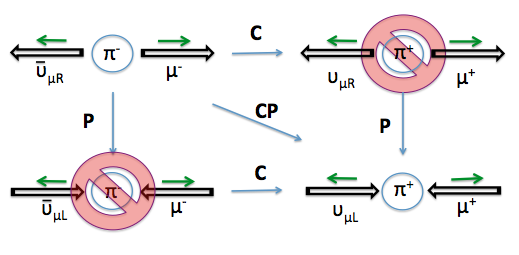
\includegraphics[scale=0.5]{figures/pion_cp}
  \caption{An illustration of the possible decays of a pion. The black arrow represents the spin vector and the green arrow represents the momentum orientation.}
  \label{fig:cp}
\end{figure}

%The convention adopted for the polarization of the muons is such that the negative muons that are polarized along their lab momentum are called \emph{forward negative muons}, while the ones that are polarized opposite to their lab momentum are \emph{ backward negative muons}. In the same way, the positive muons that are polarized opposite to their lab momentum are called \emph{forward positive muons}, while the ones that are polarized along their lab momentum are \emph{backward positive muons}.   \\  

\subsection{Parity Violation}
\label{sec:pv}
While parity is a conserved quantity in electromagnetic and strong interactions, it is not conserved in the weak interactions. 
In fact, the muon weak decays
\begin{equation}
\begin{split}
&\mu^- \rightarrow {e^-} + \bar{\nu_e} + \nu_{\mu}\\
&\mu^+ \rightarrow {e^+} + \nu_e + \bar{\nu_{\mu}}
\label{eq:decay}
\end{split}
\end{equation}
are parity violating events, which means that the emitted electrons\footnote{Unless specified, electron refers to both the electron and its antiparticle, the positron.} have a favored direction of emission. 
%This can be seen by letting $P$ act on the total angular momentum $\overrightarrow{J}=\overrightarrow{L}+\overrightarrow{S}$ before and after the decay, where $\overrightarrow{L}$ is the orbital angular momentum and $\overrightarrow{S}$ is the spin angular momentum. In the muon rest frame (MRF), $\overrightarrow{L} = 0$ so $\overrightarrow{J}=\overrightarrow{S}$. Since $\overrightarrow{S}$ is an axial vector, it is symmetric under P and thus the initial state is symmetric. After the decay, the muon spin is carried by the electron\footnote{Unless specified, electron refers to both the electron and its antiparticle, the positron.} because the neutrino and antineutrino have opposite spins that lead to their cancellation. However, the electron also has a momentum in the MRF which is antisymmetric under parity transformation since it is a vector. The final state is thus antisymmetric which confirms that the muon decay is a parity violating process.  
Because of parity violation in weak processes, a correlation exists between the momentum direction of the decaying electron and the spin orientation of the muon. In other words, there is a preferred direction for the decay of the electron for each spin orientation of the muon. For an illustration of this correlation, the negative muon decay is considered in the two limiting cases shown in Figure~\ref{fig:muon} in the muon rest frame (MRF). In the laboratory frame, the muon momentum and spin are parallel and directed to the right in the figure. \\
 \begin{figure}
  \centering
  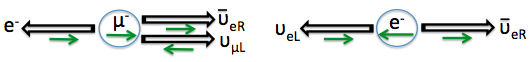
\includegraphics[scale=0.5]{figures/mu_decay}
  \caption{ In the laboratory frame, the muon spin and momentum are parallel and directed to the right. Both decays are in the MRF and show the more likely electron direction. The left decay shows an electron having the maximum possible energy $E_{e,max}\sim \left(m_{\mu}c^2\right)/2$ = 53 MeV. The right decay shows an electron emitted at rest with its spin antiparallel to its laboratory momentum. }
  \label{fig:muon}
\end{figure}
If the electron has the maximum possible energy in the MRF, the two neutrinos will be emitted back-to-back to the electron with the latter carrying half of the rest mass energy of the muon in order to conserve momentum, $E_{e,max}\approx \left(m_{\mu}c^2\right)/2$ = 53 MeV. 
%The neutrino-antineutrino pair carries zero spin (since the left-handed neutrino is parallel to the right-handed antineutrino), the spin angular momentum of the muon is carried by the electron.
Parity violation favors the electron to be emitted left-handed which implies that its momentum will be anti-parallel to the muon spin as shown in the left figure. In the case of a zero momentum electron in the MRF, the neutrino and antineutrino will be emitted antiparallel to each other with their spins parallel. Since the electron has a preferred spin direction antiparallel to the muon laboratory momentum and the muon momentum and spin are parallel. The electron will be emitted parallel to the muon spin as shown on the right figure. These two examples show that by knowing the direction of the decay electron, the muon spin orientation can be inferred. This is the key idea of the muon $g-2$ measurement. By placing muons with the same polarization in a circular orbit with a uniform magnetic field, their longitudinal polarization\footnote{Longitudinal polarization refers to the spin component parallel to the momentum vector.} will change slightly with each orbit at a rate that is directly related to the anomaly $a_{\ell} = \frac{g_\ell-2}{2}$. The change in the muon longitudinal polarization is determined by using the asymmetric angular distribution of the decay electrons. Formally, the differential decay probability for an electron to be emitted with a normalized energy $y=E/E_{e,max}$ at an angle $\theta$ with respect to the muon spin is given in the MRF with the approximation $E_e \gg m_e c^2$ by
\begin{equation}
dP^{\pm} \propto N\left(E_e\right)\left(1 \pm A(E_e)\cos \theta \right) dy d\Omega
\label{eq:prob}
\end{equation}
where the $(+)$ is for positive muon decay and the $(-)$ is for negative muon decay and $d\Omega$ is the solid angle. $N\left(E_e\right)$ is a normalization factor that represents the number of decay electrons per unit energy and $A\left(E_e\right)$ is the non-vanishing coefficient of $\cos \theta$ which represents the decay asymmetry factor that reflects the \emph{parity violation}. Their expressions are given by
\begin{equation}
N\left(E_e\right) = 2y^2\left(3-2y\right)  \,\,  \text{and}  \,\,  A\left(E_e\right) = \frac{1-2y}{3-2y}.
\label{eq:na}
\end{equation}
These relations are derived in Appendix \ref{app:muon}.

Few remarks related to equations \ref{eq:prob} and \ref{eq:na} are in order. First, the number and asymmetry reach their highest values in the MRF when the energy of the emitted electron is maximum ($y=1$) as shown in Figure \ref{fig:CMF}
 \begin{figure}
    \centering
  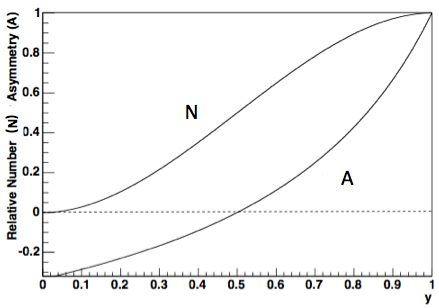
\includegraphics[scale=0.5]{figures/CMF}
   \caption{Muon Rest Frame: The number of decay electron and the asymmetry distributions, given by equations \ref{eq:na} in the MRF, as a function of the fractional energy $y=E/E_{e,max}$ where $E_{e,max} \approx 53 \text{MeV}$ \cite{bnl}}
  \label{fig:CMF}
\end{figure}
Also, the asymmetry changes sign at half the maximum energy ($y=\frac{1}{2}$) which means that the emitted electron will have a preferred handedness (or helicity) based on its energy. More importantly, the probability of emitting a specific number of electrons varies with the angle $\theta$ between the electron and the muon spin directions. To be precise, there are more high energy electrons ($e^-$) emitted when their momenta are anti-parallel to the muon ($\mu^-$) spins than when they are parallel. For example, by only selecting the highest energy electrons and counting their number, the spin direction of the muons can be inferred; when the number of electrons is maximum, the muon spin is anti-parallel to the emitted electron direction, and when the number is minimum, the muon spin is parallel to the emitted electron direction. A similar reasoning can be followed for high energy positrons ($e^+$) which will reach a maximum number when the positive muon ($\mu^+$) spins are parallel to the emitted positrons. If the spin of the muons is made to precess, as it will be discussed in the next section, then the number of high energy electrons will also precess at the same rate allowing a direct measurement of this precession. 

\subsection{Relativistic Muons in a Magnetic Field}

By invoking classical imagery, it can be seen that the effect of a uniform magnetic field on a bar magnet is to exert a torque that will align the magnet with the magnetic field. However, if the magnet is spinning, then conservation of angular momentum will cause the bar magnet to precess around the magnetic field. Similarly, the muon has an intrinsic spin and an intrinsic magnetic moment. The interaction of the muon magnetic moment with the magnetic field will cause a precession of the spin around the magnetic field. In fact, it is the expectation value of the spin operator
%\footnote{expectation value vocabulary} 
that precesses around the magnetic field at a constant frequency known as \emph{Larmor frequency}. 
This frequency describes the gyration of the spin and is proportional to the magnetic field, thus the name of \emph{gyromagnetic ratio} $g$. 

%The Larmor angular frequency, derived in Appendix (?), is
%\begin{equation} 
%\overrightarrow{\omega_L} = -g\frac{q}{2mc}\overrightarrow{B}.
%\end{equation}

For highly relativistic muons\footnote{Muons with velocities close to the speed of light.} with a transverse acceleration\footnote{A component of acceleration normal to the velocity vector.}, a new precession is introduced that is purely kinematic due to the acceleration of the relativistic reference frame. This precession is derived in Appendix \ref{app:bmt} and is referred to by \emph{Thomas precession}.

If relativistic muons are constrained to a circular orbit by a uniform magnetic field, as it is the case in a \emph{storage ring}\footnote{A storage ring is a circular particle accelerator that maintains particles at the same energy for a long period of time}, their spins experience both Larmor and Thomas precessions. The ensemble of these effects on the spin was worked out by Bargmann, Michel and Telegdi in 1959 [\textbf{reference}], in an equation known as the BMT equation (see Appendix \ref{app:bmt})
\begin{equation}
\overrightarrow{\omega_s} =  \frac{q}{m_{\mu}c}\left\{\left(a_{\mu} + \frac{1}{\gamma}\right)\overrightarrow{B}    -   a_{\mu}\left(\frac{\gamma}{\gamma + 1}\right)\left(\overrightarrow{\beta} \cdot \overrightarrow{B}\right)\overrightarrow{\beta}   +   \left(a_{\mu}+\frac{1}{\gamma + 1}\right)\overrightarrow{E} \times\overrightarrow{\beta}                 \right\}
\end{equation}
where $\overrightarrow{\beta} = \frac{\overrightarrow{v} }{c}$, the Lorentz factor is $\gamma = 1/\sqrt{1-\beta^2}$, $\overrightarrow{E}$ and $\overrightarrow{B} $ are the electric and magnetic fields in the laboratory frame respectively.

In addition, the muons also travel in a circular orbit with a frequency known as the \emph{cyclotron frequency}:
\begin{equation}
\overrightarrow{\omega_c} = \frac{q}{\gamma m_{\mu}c}\left\{\overrightarrow{B} + \frac{\gamma^2}{\gamma^2-1} \left(\overrightarrow{E} \times \overrightarrow{\beta}\right)\right\}.
\label{eq:c}
\end{equation}

It is convenient to choose a reference frame which rotates with the velocity vector in order to keep the equations simple. In this case, the precession is given by the difference of angular frequencies $\overrightarrow{\omega_a} = \overrightarrow{\omega_s} - \overrightarrow{\omega_c}$, 
\begin{equation}
\overrightarrow{\omega_a} =   \frac{q}{m_{\mu}c}\left\{a_{\mu}\overrightarrow{B}   -   a_{\mu}\left(\frac{\gamma}{\gamma + 1}\right)\left(\overrightarrow{\beta} \cdot \overrightarrow{B}\right)\overrightarrow{\beta} +   \left(a_{\mu}-\frac{1}{\gamma^2 - 1}\right)\overrightarrow{E} \times\overrightarrow{\beta}                 \right\}
\label{eq:bmt}
 \end{equation}
If the second and third terms are made to vanish by a proper choice of muon momenta and applied electric and magnetic fields, then equation \ref{eq:bmt} becomes
\begin{equation}
\overrightarrow{\omega_a} =   a_{\mu}\frac{q}{m_{\mu}c}\overrightarrow{B} 
\label{eq:wa}
\end{equation}
In this case, $a_{\mu}$ is directly responsible for the precession of the muon spin relative to the cyclotron frequency. This is the central equation of the $g-2$ experiment that will be discussed in the next section. 


\section{The Muon $g-2$ Experiments}
The muon magnetic moment has been measured by three consecutive experiments at CERN through the 60's and 70's, and a more recent experiment at Brookhaven National Laboratory (BNL), E821. The last CERN experiment developed a number of novel techniques to measure the anomaly. For instance, it employed a storage ring with a transverse uniform magnetic field to extend the muon's lifetime and cancel the first term in equation \ref{eq:bmt} since $\overrightarrow{\beta} \cdot \overrightarrow{B} = 0$. The experiment chose a specific momentum according to the relation $a_{\mu} -1/\left(\gamma^2-1\right) = 0$ in equation  \ref{eq:bmt} known as the \emph{magic momentum}, which causes the spin oscillation to be independent of any applied electric fields. The goal of this experiment was to measure the anomaly to a very high precision, but its value was measured by previous experiments to the first few decimal placements. An anomaly value of $a_{\mu} \approx 1.166\times 10^{-3}$ led to a Lorentz factor value of $\gamma_{\text{magic}} \approx 29.30$, and thus the magic momentum is approximately 3.09 GeV in the CERN experiment. 
At the magic momentum, electric quadrupoles\footnote{Electric quadrupole is a system composed of two pairs of oppositely polarized poles placed antiparallel to each other.} were used to provide vertical focusing of the beam. The combined results of the CERN run established a 7.3 ppm precision that was consistent with the standard model prediction. The new measurement techniques developed at CERN were used at Brookhaven with some notable improvements such as the higher intensity of the primary proton beam from the proton storage ring, the direct injection of muons into the storage ring instead of pions, the use of kickers to place muons on the correct orbits, the  high field uniformity and the use of NMR probes to map the magnetic field distribution. The E821 experiment resulted in a 14-fold improvement over the CERN experiment where it performed four positive muon runs and one negative muon run which gave a combined precision of 0.54 ppm. In this section, a description of the E821 experiment and the summary of its measurements is given along with the improvements that are expected to take place with its upgrade E989 at Fermilab.\\

\subsection{BNL E821 $g-2$ Experiment}

\textbf{Description of the Experimental Method}

At BNL, 24 GeV protons are extracted from the proton storage ring AGS (Alternating Gradient Synchrotron) and directed towards a nickel target to generate pions. The pions subsequently decay to muons which pass through selectors that maximize the number of longitudinally polarized muons at the magic momentum of 3.094 GeV/c. These muons are injected into the storage ring via a tangent 1.7 meters long superconducting inflector magnet that provides a 1.5 Tesla vertical field that cancels the main storage ring field, allowing the muons to pass almost undeflected into the ring. The muon storage ring has a toroid-shaped structure with a diameter of 14 meters, a beam pipe with a diameter of 90 mm, and a uniform field of 1.45 Tesla. This magnetic field is provided by dipole magnets\footnote{A dipole magnet is a configuration of two opposite pole magnets in the vertical plane of the ring which provide a transverse magnetic field.} that maintain muons in the desired trajectories. However, when the muons are first injected, their trajectories are offset from the storage ring orbit. Pulsed kicker magnets are placed at a specific location in the ring, close to the inflector exit in order to apply a small magnetic field, a ``kick", to adjust the orbit by approximately 10 mrad on each pass. Figure \ref{fig:chain} shows the complete chain of the muon $g-2$ experiment at BNL for positive muons.
 \begin{figure}
    \centering
  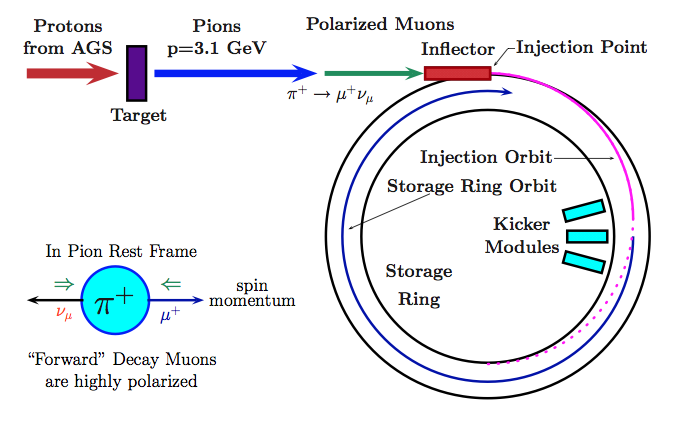
\includegraphics[scale=0.39]{figures/chain}
   \caption{The chain of injection and storage of positive muons in the muon $g-2$ ring at BNL. The ``forward'' muons refer to muons decaying in the same direction as the laboratory momenta. In this situation, positive muons have their spins anti-parallel to their momenta. \cite{phen}}
  \label{fig:chain}
\end{figure}

Beam focusing is also needed to constrain the muons to the desired trajectories. Since electric fields do not affect the spin precession, electrostatic quadrupoles are used to continuously focus and defocus the beam in the vertical and the horizontal directions in order to precisely control the beam. 

Muons will travel around the ring at the cyclotron angular frequency described by equation \ref{eq:c} and their spin will interact with the magnetic field resulting in a precession with the angular frequency $\omega_s$ given by equation \ref{eq:bmt}. However, the electric field $\overrightarrow{E}$ is negligible ($E \approx 0$) and the uniform magnetic field is transverse ($\overrightarrow{\beta} \cdot \overrightarrow{B} = 0$), so the anomalous precession frequency, $\overrightarrow{\omega_a}$, is given by equation \ref{eq:wa} to first order. Its magnitude is  
\begin{equation}
\omega_a =   a_{\mu}\frac{eB}{m_{\mu}c} 
\label{eq:waa}
\end{equation}

If $g = 2$, then this relative precession $\omega_a$ will be zero, which implies that the muon spin is precessing at the same frequency as the cyclotron frequency. On the other hand, if $g \neq 2$, the muon spin will precess at a higher rate than the cyclotron frequency, leading the muon spin axis to change by 12 arcseconds\footnote{1 degree = 3600 arcseconds.} after each rotation for a constant momentum. Figure \ref{fig:ring} illustrates this change by showing the momentum vector and the projection of the spin vector in the horizontal plane of the storage ring. 
\begin{figure}
  \centering
  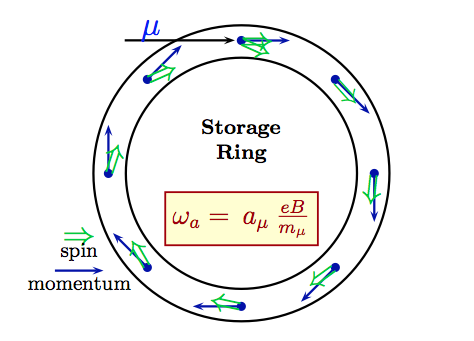
\includegraphics[scale=0.5]{figures/ring}
  \caption{Illustration of the spin precession in the storage ring plane relative to a constant momentum (Not to scale). The precession amounts to $\sim$ 12 arcseconds per each orbit.  \cite{phen}}
  \label{fig:ring}
\end{figure}
 
In order to determine the anomaly $a_{\mu} = \frac{g_{\mu}-2}{2}$, three quantities need to be determined accurately: $\omega_a$, $B$, and the muon mass $m_{\mu}$. The muon mass will be determined indirectly by an independent experiment on muonium, the bound state of $\mu^+e^-$. The next two sections describe the measurement of $\omega_a$ and the magnetic field B.

\textbf{Measurement of $\omega_a$}

As a result of the muons high momentum ($\sim$ 3.1 GeV), their lifetime is extended from $\tau_{\mu}$ = 2.1971 $\mu s$ at rest to 64.435 $\mu s$ (theory). The muons circle the ring many times before they decay into an electron and two neutrinos given by equation \ref{eq:decay}. As discussed in section \ref{sec:pv}, the electron has a preferred emission direction in the muon rest frame, that depends on the orientation of the muon spin as given by equation \ref{eq:prob}. For example, a positron has a higher probability to be emitted parallel to the muon spin (see Figure \ref{fig:det}). 
\begin{figure}
  \centering
  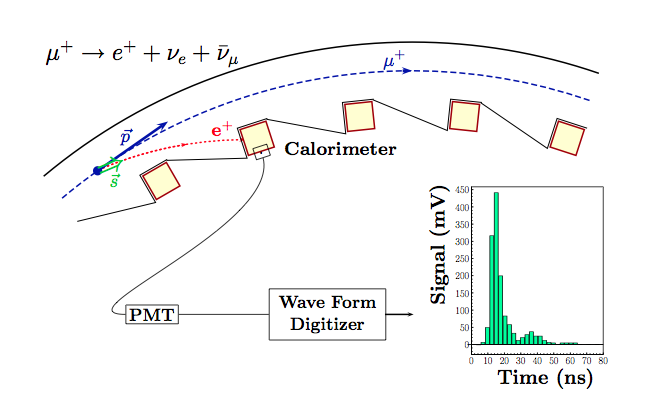
\includegraphics[scale=0.5]{figures/detection}
  \caption{A positive muon in the storage ring emits a positron almost parallel to the muon spin (green arrow). The electron is subjected to the same dipole magnetic field which produces a larger deflection leading the positron to interact with the calorimeter scintillator. The light is detected by a Photomultipler Tube (PMT) generating a signal that is digitized by a Wave Form Digitizer. \cite{phen}}
  \label{fig:det}
\end{figure}


If all decay electrons were detected, the number observed will decay exponentially as $\exp(\frac{-t}{\gamma \tau_{\mu}})$. Since the interest is in the precession frequency, a choice of a cut on a laboratory observable is required so that only a subset of the decay electrons are selected in such a way that their number oscillates at the desired frequency $\omega_a$. The direction of the electron cannot be chosen as a cut since electrons near the magic momentum, $p_{\mu} \approx 3.09 GeV/c$, have a direction that is almost parallel to the muon momentum direction, irrespective of their decay orientation in the muon rest frame. A more practical cut can be applied on the electron's laboratory energy for the reasons given in section \ref{sec:pv}. For instance, if only electrons with the highest possible energy are selected, they will represent positrons that decayed nearly parallel to the muon laboratory momentum with maximum muon rest frame energy. The number of these positrons is larger when they are emitted parallel to the muon spin as opposed to when they are antiparallel. So the number of positrons detected will be maximum when the spin is aligned with the decay positron momentum, and will be minimum when the spin is opposite. It becomes clear that the detected electrons will oscillate with the frequency of the muon spin oscillation $\omega_a$.

In practice, the selected minimum energy threshold is E$_{th}\approx$ 1.8 GeV ($y\approx.58$) which corresponds to the laboratory energy above which electrons have a more probable decay direction as shown in Figure \ref{fig:LAB}. 
%figure out a way to have figures next to each other.
\begin{figure}
  \centering
  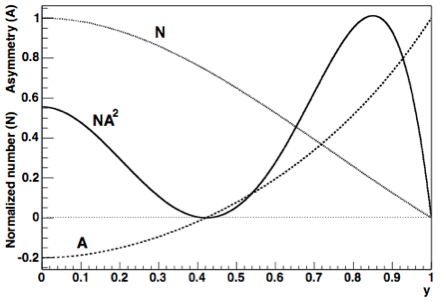
\includegraphics[scale=0.5]{figures/LAB}
   \caption{The equivalent of Figure \ref{fig:CMF} boosted to the laboratory frame. The fractional energy is $y=E/E_{e,max}$ where $E_{e,max} \approx 3.098$ GeV. The quantity $NA^2$ represents the \emph{statistical figure-of-merit}. It needs to be maximized in order to achieve a minimum statistical uncertainty. \cite{bnl}}
  \label{fig:LAB}
%  \caption{The number of decay electron and the asymmetry distributions, given by equations (\ref{eq:na}) in the MRF, as a function of the fractional energy $y=E/E_{e,max}$ where $E_{e,max} \approx 3.094 \text{GeV/c}$}
\end{figure}
With the the assumption that the spin precession vector is independent of time, the angle between the spin component in the orbit plane and the muon momentum is $\omega_at+\phi$, where $\phi$ is a constant phase. At time t, the number of decay positrons N(t) with energy larger than the threshold energy E$_{th}$ is
\begin{equation}
N(t, E_{th}) = N_0(E_{th})\exp \left(\frac{-t}{\gamma \tau_{\mu}}\right) \left[1 + A(E_{th})  \sin\left(\omega_a t + \phi(E_{th})\right)\right],
\label{eq:fit}
\end{equation}
where N$_0$ is a normalization factor and A is the asymmetry factor for positrons of energy greater than E$_{th}$. 

 \begin{figure}
  \centering
  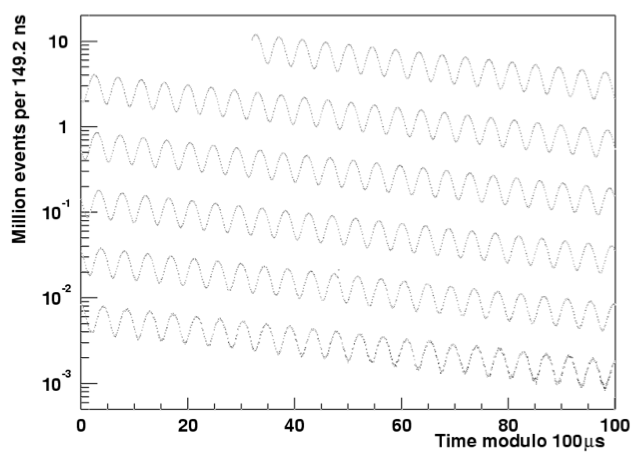
\includegraphics[scale=0.5]{figures/oscillation}
  \caption{Histogram of the 3.6 billion detected electrons above 1.8 GeV as a function of time, modulo 100 $\mu s$, for the 2001 data set \cite{bnl}.}
  \label{fig:osc}
\end{figure}
Figure \ref{fig:osc} shows the arrival-time spectrum of the final E821 data run for 2001. As discussed, the spectrum follows an exponential decay of the muons modulated by the $g-2$ dependent angular frequency. By fitting this time distribution to the five-parameter function of equation \ref{eq:fit}, the angular frequency $\omega_a$ is determined.

The electron detection is made via 24 symmetrically distributed calorimeters in the inside of the ring as shown in Figure \ref{fig:det}. The goal of the calorimeters is to determine the electrons energy and arrival time. The calorimeters are designed to detect the high energy electrons where 65 percent of the electrons with energy higher than 1.8 GeV are intercepted \cite[p.~29]{bnl}. Each calorimeter is made out of plastic-scintillator\footnote{A particle deposits energy when it passes through a plastic-scintillator, the latter re-emits the absorbed energy in the form of light. } material (52\% lead alloy, 38\% scintillating fiber, and 10\% epoxy) read out by photomultiplier tubes\footnote{Photomultiplier tubes are light detectors that operate via the photoelectric effect where a single photon, upon hitting a photocathode, generates a cascade of electrons that can be read by a Wave Form Digitizer.} (PMTs). The decaying electrons have both a tangential and radial momentum components. However, the radial component is quite small which permits the extrapolation of the electron's trajectory from the calorimeter to the central muon orbit, allowing a measurement of the decay position and vertical angle as shown in Figure \ref{fig:det}. The muon position information is particularly important in characterizing the magnetic field felt by the muon at that specific location. 
% BNL p34 
Finally, a Wave Form Digitizer (WFD) captures raw analog PMT signals and digitize them for further processing with the advantage of maintaining high resolution measurements. An example of a WFD output is shown in Figure \ref{fig:det}.

\textbf{Measurement of the magnetic field B}

The magnetic field B is weighted by the stored muons distribution and averaged over the running time. It can be expressed as an integral of the product of the muon distribution times the magnetic field distribution over the storage region leading to a coupling of the moments of the muon distribution to the respective multipoles of the magnetic field. In order to determine the weighted B to sub-ppm precision, either the moments and multipoles of the muon and magnetic field distributions should be known extremely well, or a particularly uniform magnetic field and a circular beam aperture is required to have the leading term dominate the multipole expension of the magnetic field. The latter option was selected where \emph{Nuclear Magnetic Resonance} (NMR) permitted the determination of the magnetic field to the tens of ppb. In this experiment, NMR is based on using protons in a water sample placed in the dipole magnetic field, and exposed to a $\frac{\pi}{2}$ radio-frequency (RF)\footnote{Radio-frequency ranges from 3 KHz to 300 GHz.} pulse which rotates the net magnetization of the protons. A pickup coil placed in the transverse direction registers the induced signal that exponentially decays with an oscillation as the protons' magnetization regains its equilibrium position. The latter process, known as \emph{Free Induction Decay}, has a frequency sensitive to the the local magnetic field value. This procedure allows the determination of the magnetic field at thousands of points around the ring which permits the mapping and monitoring of the field during data taking. A calibration method is used to express the Larmor spin frequency of a proton in a water sample in terms of the Larmor spin frequency of a free proton $\omega_p$. The latter frequency, $\omega_p$, is related to the magnetic moment of the free proton $\mu_p$ and the magnetic field B by\footnote{The Larmor frequency of a free proton is $\omega_p=\gamma_pB$, where $\gamma_p$ is the free proton gyromagnetic moment ratio given by equation \ref{eq:mu} such that $\overrightarrow{\mu_p} = \gamma_p \overrightarrow{S}$. These relation give the result in equation \ref{eq:wp}}
\begin{equation}
B = \frac{\hbar\omega_p}{2\mu_p}.
\label{eq:wp}
\end{equation} 
According to the last equation, this weighted magnetic field can be referred to as $\omega_p$. 
By writing equation \ref{eq:mu} in the form $\displaystyle \frac{q}{mc} = \frac{2\mu_{\mu}}{1+a_{\mu}}$ and using equations \ref{eq:waa} and \ref{eq:wp}, the anomaly can be written in terms of dimensionless ratios,
\begin{equation}
a_{\mu} = \frac{\mathcal{R}}{\lambda - \mathcal{R}},
\label{eq:R}
\end{equation}
where $\displaystyle \lambda \equiv \frac{\mu_{\mu}}{\mu_{p}}$ and $\displaystyle \mathcal{R} \equiv \frac{\omega_a}{\omega_p}$.
The muon-to-proton magnetic moment ratio, $\lambda$, embodies in it both the muon and the proton masses since $\displaystyle \frac{\mu_{\mu}}{\mu_{p}} = \frac{g_{\mu}}{g_p}\frac{m_p}{m_{\mu}}$. Its value is determined through a precision measurement of the Zeeman ground state hyperfine transitions in muonium ($\mu^+e^-$) by E1054 LAMPF at Los Alamos \cite{zeeman},
\[\lambda_+ = \frac{\mu_{\mu^+}}{\mu_{p}} = 3.183\, 345\, 137\, (85).\] %check value in CODA ?
Note that this result has a precision of $\sim 27$ ppb which could not be obtained by mass measurements. The use of $\lambda_+$ to determine $a_{\mu^-}$ implies CPT invariance\footnote{CPT invariance refers to the assumption that physical processes are invariant under a charge (C), parity (P), and time (T) transformation.}. In other words, the relations $a_{\mu^-} = a_{\mu^+}$ and $\lambda_+ = \lambda_-$ must be valid. In fact, the measurement of $\omega_a$ for positive and negative muons provides a CPT test where 
\begin{equation}
\Delta \mathcal{R} = \mathcal{R}_{\mu^-} - \mathcal{R}_{\mu^+} = \left(3.6 \pm 3.7 \right) \times 10^{-9}.
\end{equation}

\textbf{Corrections and systematic errors}

The method described so far presents an ideal scenario. However, there are additional effects that affect the measurements, the most important of which will be described in this section.  
While the dipole magnetic field insures the bending of the muon beam, the vertical focusing is done via electric quadrupoles. These quadrupoles set an electric field gradient that causes the beam to oscillate around its equilibrium in the plane transverse to the beam. This type of oscillation is known as the \emph{betatron oscillation} and it satisfies the harmonic oscillator equations 
\begin{equation}
\begin{split}
\ddot{x} + \omega_x^2 x = 0, \\
\ddot{y} + \omega_y^2 y = 0,
\end{split}
\end{equation}
with the frequencies 
\begin{equation}
\begin{split}
\omega_x = \omega_c\sqrt{1-n} \,\,\,\,\,\,\,\,
\omega_y = \omega_c\sqrt{n}
\end{split}
\end{equation}
where $ \omega_c$ is the cyclotron frequency and n is the field index defined as 
\begin{equation}
n = \frac{R_0}{\beta B_0}\frac{\partial E_y}{\partial y}
\end{equation}
with an orbit stability condition of $0<n<1$ and $R_0$ is the equilibrium radius, $B_0$ is the dipole magnetic field, and $\beta$ is the muon speed. Since the betatron frequencies are smaller than the cyclotron frequency, this type of focusing is called \emph{weak focusing}.
 
The betatron motion perturbs the muon trajectories affecting their momenta and directions. This implies that the assumptions $\overrightarrow{\beta} \cdot \overrightarrow{B} = 0$ and $a_{\mu} -1/\left(\gamma^2-1\right) = 0$ ($E \approx 0$) are no longer valid. These effects should be taken into account in determining the anomalous frequency $\omega_a$ as given by equation \ref{eq:wa}. The correction for the momentum direction to satisfy $\overrightarrow{\beta} \cdot \overrightarrow{B} = 0$ is called the \emph{Pitch Correction}. Similarly, the momentum spread from the magic momentum requires a correction to the electric field referred to as the \emph{Radial Electric Field Correction}. The combination of these two corrections are explicitly shown in column 2 of Table \ref{tab:R}. 

Next, the sources of systematic errors in $\omega_a$ are briefly defined with their numerical values listed in Table \ref{tab:sys}:
\begin{itemize}
\item Pileup: Two low-energy electrons that reach the detector at very close times can be interpreted as one high-energy electron.        
\item AGS background: Mis-steered proton beam in the AGS might hit a part of the target that produces a high flux of pions entering the storage ring when muons are injected. %p11
\item Lost Muons: Small perturbations in the magnetic or electric fields may couple to betatron oscillations at their resonant frequency leading to a motion without bound until the muons are lost.
\item Timing Shifts: Time resolution of the detector. % PMT 
\item Fitting/Binning: Errors associated with the multi-parameter fitting function and the binning of the electron decay spectra. 
\item Coherent Betatron Oscillation (CBO): Oscillations that result from the mismatch between the inflector and storage ring apertures imposing a narrow waist at injection. %p41
\item Gain Changes: Variations in the energy scale used for detected electrons.
\end{itemize}
\begin{table}
  \caption{ Systematic errors for $\omega_a$ for the three high-statistics running periods. ${\dagger}$In the 2001 run, the AGS background, timing shifts, E field and pitch correction, binning and fitting procedure have a total systematic error of 0.11ppm. }
  \label{tab:sys}
  \centering
  \begin{tabular}{*{4}{l}}
	\hline \hline
      Years   & 1999 & 2000  & 2001 \\ 
      %$\sigma_{sys}$($\omega_a$)
       & (ppm) & (ppm) & (ppm)\\
      \hline
       Pileup & 0.13 & 0.13 & 0.08  \\
       AGS background & 0.10 & 0.01 &    ${\dagger}$\\
       Lost Muons & 0.10 & 0.10 & 0.09  \\
       Timing Shifts & 0.10 & 0.02 &    ${\dagger}$\\
       E-field and pitch & 0.08 & 0.03 &    ${\dagger}$\\
       Fitting/Binning & 0.07 & 0.06 &    ${\dagger}$\\
       CBO  & 0.05 & 0.21 & 0.07  \\
       Gain Changes & 0.02 & 0.13 & 0.12   \\ \hline
       Total systematic error on $\omega_a$ & 0.3 & 0.31 & 0.21  \\
         \hline  \hline
     \end{tabular}
\end{table}

The systematic uncertainties in the magnetic field measurement are due to effects related to the determination of the precession frequency of protons in a water sample placed in a trolley probe that is offset from the orbit of the muons. The positioning of the trolley permits measurements of the magnetic field during data taking at multiple locations around the ring. However, the trolley's position sees a magnetic field that might vary from the field that muons experience. In addition, the proton precession frequency is measured in water while the required quantity is the free proton precession. For these reasons, uncertainties are introduced in the processes of calibration and interpolation. Table \ref{tab:wp} summarizes the numerical values of the errors for three running periods.
\begin{table}
  \caption{ Systematic errors for $\omega_a$ for the three high-statistics running periods. $\dagger$ After 1999, the inflector, which was damaged, was replaced making the disturbance of the inflector's fringe field on the main storage ring field negligible.}
  \label{tab:wp}
  \centering
  \begin{tabular}{*{4}{l}}
	\hline \hline
      Years   & 1999 & 2000  & 2001 \\ 
      %$\sigma_{sys}$($\omega_a$)
       & (ppm) & (ppm) & (ppm)\\
      \hline
       Absolute calibration of standard probe & 0.05 & 0.05 & 0.05  \\
       Calibration of the trolley probes & 0.20 & 0.15 & 0.09 \\
       Trolley measurements of B & 0.10 & 0.10 & 0.05  \\
       Interpolation with fixed probes & 0.15 & 0.10 &  0.07 \\
       Uncertainty from muon distribution & 0.12 & 0.03 & 0.03 \\
       Inflector fringe field uncertainty & 0.20 & $\dagger$ &  $\dagger$  \\
       Others  & 0.15 & 0.10 & 0.10     \\ \hline
       Total systematic error on $\omega_p$ & 0.4 & 0.24 & 0.17 \\ \hline  \hline
     \end{tabular}
\end{table}

The electric dipole moment (EDM) of the muons should also be mentioned for completeness of the discussion. Just as the magnetic moment originates from the current of the spinning charged lepton and interacts with the magnetic field, the EDM is due to the electric charge of the lepton and it interacts with the electric field. The equivalent of equation for the EDM is  
\begin{equation}
\overrightarrow{d} = \eta\frac{q}{2mc}\overrightarrow{S}
\label{eq:d}
\end{equation}
where $d$ is the dimensionless constant equivalent to the g-factor. Its current experimental value for muons is $d_\mu = \left(-0.1 \pm 0.9\right) \times 10^{-19} e \cdot \text{cm}$ [PDG], which is too small to affect the anomalous precession frequency $\omega_a$.

\textbf{Results from E821}

E821 has conducted four positive muon runs (1997-2000) and one negative muon run (2001) that are all reported in \cite{bnl}. The results of the experiment for the last three runs are displayed in Tables \ref{tab:R} and \ref{tab:amu}.
\begin{table}
  \caption{Results for the anomalous precession frequency $\omega_a$ including the relative electric field and pitch corrections shown in column 2 and the event-weighted magnetic field $\omega_p$ given with their uncertainties. The error on the average takes into account the correlated systematic uncertainties between different periods.}
  \label{tab:R}
  \centering
  \begin{tabular}{*{6}{c}}
	\hline \hline
      Years  & Electrons & $\omega_a/(2\pi)$& E/pitch & $\omega_p/(2\pi)$ & $\mathcal{R} = \omega_a/\omega_p$\\ 
      &[millions] &  [Hz]  &  [ppm]  & & \\
      \hline
       1999 ($\mu^+$) & 950 & 229\,072.8(3) & 0.81(8) & 61\,791\,256(25)& 0.003\,707\,204\,1(51)  \\
       2000 ($\mu^+$) & 4000 & 229\,074.11(16) & 0.76(3) & 61\,791\,595(15)& 0.003\,707\,205\,0(25)  \\
       2001 ($\mu^-$)  & 3600 & 229\,073.59(16) & 0.77(6) & 61\,791\,400(11)& 0.003\,707\,208\,3(26)  \\  \hline
       Average & & & & & 0.003\,707\,206\,3(20) \\
         \hline  \hline
     \end{tabular}
\end{table}
\begin{table}
  \caption{BNL E821 results of the anomaly $a_{\mu}$ for the three high-statistics running periods. }
  \label{tab:amu}
  \centering
  \begin{tabular}{*{4}{c}}
	\hline \hline
      Years  & Polarity & $a_{\mu}\times 10^{10}$ & Precision [ppm] \\ \hline
       1999 & $\mu^+$ & 11\,659\,202(15) & 1.3  \\
       2000 & $\mu^+$ & 11\,659\,204(9) & 0.73  \\
       2001 & $\mu^-$ & 11\,659\,214(9) & 0.72  \\ \hline
       Average & & 11\,659\,208.0(6.3) & 0.54\\
         \hline  \hline
     \end{tabular}
\end{table}

The averaged value of the ratio $\mathcal{R} = \omega_a/\omega_p$ of equation \ref{eq:R} evaluated in the cases of negative and positive muons is
%\begin{equation}
%\begin{split}
%\mathcal{R}_{\mu^+} = 0.003\,707\,204\,7(26)
%\mathcal{R}_{\mu^-} = 0.003\,707\,208\,3(26)
%\end{split}
%\end{equation}
%giving the average value
\begin{equation}
\mathcal{R}_{\mu}\left(\text{E821}\right) = 0.003\,707\,206\,4(20).
\end{equation}
The anomalous magnetic moment is thus 
\begin{equation}
a_{\mu}^{\text{E821}} = 11\, 659\, 208  \left(5.4\right)_{stat}  \left(3.3\right)_{sys}  \left(6.3\right)_{tot} \times 10^{-10} \,\,\,\,\,\,\, \left(0.54  \text{ ppm}\right)
\end{equation}
This final measurement has a statistical uncertainty of 0.46 ppm and a systematic uncertainty of 0.28 ppm which were added in quadrature to get a total uncertainty of 0.54 ppm. In order to improve the statistical uncertainty, which dominates the measurement, an additional running period of 8 years is required. Alternatively, the experiment can use a higher intensity beam to produce more electrons, and thus more statistics. This is precisely what the new Fermilab experiment does.

\subsection{Future Fermilab $g-2$ Experiment: E989}

The Fermilab experiment, E989, will measure the anomaly $a_{\mu}$ with an error of $1.6 \times 10^{-10}$ leading to a fractional error of 0.14 ppm, where the level of the statistical and systematic uncertainties are both at the 0.10 ppm level. In order to achieve this goal, a collection of data that is twenty-one times larger than the E821data collection is required, which scales to $1.8\times10^{11}$ detected positrons with energy greater than 1.8 GeV, and arrival time greater than $30 \mu s$ after muon injection in the storage ring. Since the detected positron number is directly proportional to the protons on target, the Fermilab experiment will have to deliver $4\times10^{20}$ protons. Indeed, it will be possible to reach these numbers by using the Fermilab beam complex which is expected to annually deliver $2.3 \times 10^{20}$ 8 GeV protons on an Inconel\footnote{Inconel is an alloy, composed of a metal and other elements, specifically designed to withstand high beam stresses.} core target. At this rate, the desired number of protons, and thus positrons, will be achieved in less than two years of running. \\
Fermilab will improve upon the methods and instrumentation used at BNL. For instance, the produced pion beam will pass through a bending magnet to select particles with a momentum of 3.1 GeV ($\pm$ 10 \%), and subsequently traverse a decay line of over one kilometer, which leads to a pure muon beam entering the storage ring. The muon storage ring will be filled at a repetition rate of 15 Hz compared to 4.4 Hz at BNL, and the stored muon-per-proton ratio will also be increased by a factor of 5 to 10 times. The muons will enter the ring via a new superconducting inflector, characterized by a limited flux leakage onto the storage region and a larger horizontal beam aperture to allow a higher storage efficiency. The muon kicker will have an optimized pulse-forming network\footnote{Pulse-forming network is an electric circuit composed of capacitors that provide a square pulse with a flat top upon discharge.} that provided a pulse close to the beam width, as opposed to the E821 quicker which had a pulse width longer than the cyclotron period. At BNL, the injected muon beam was contaminated with pions which introduced a hadronic flash background. This background will be reduced by a factor of 20 in E989. \\
E989 will use the same muon storage ring of E821, which has been relocated to Fermilab in the summer of 2013 in a new building characterized by mechanical stability and controlled temperature. These options were not available at BNL.\\
The new segmented calorimeters will use silicon Photomultipliers (SiPMs) to read signals from lead-fluoride crystal (PbF$_2$). The crystal has an improved energy resolution and a very fast Cherenkov signal\footnote{Cherenkov signal is due to Cherenkov radiation which is an electromagnetic radiation produced when a particle travel through a dielectric material with a velocity greater than the phase velocity of light in that dielectric. While no particle travels faster than light in vacuum, the situation is different in a dielectric since $v_\text{light}$ = c/n with n $>$1.} response. When a photon strike a SiPM pixel, it generates an avalanche that is linearly combined with the other pixels that were hit to form the response. SiPMs are designed so that their number of pixels exceed the number of photons that are expected to strike the device allowing a high photo-detection efficiency. The added benefit of using SiPMs is that they can be placed inside the storage ring at the back of the PbF$_2$ crystals without perturbing the field, as opposed to PMTs which require long lightguides. \\
Since momentum spread, betatron oscillations, and muons distribution introduced ppm level corrections in the anomalous precession at BNL, E989 introduces in-vacuum straw drift tubes\footnote{A straw tube for high resolution position measurement is constructed with an anode wire centered within a cathode tube and maintained at a potential difference in a gas environment.  When a charged particle passes through the tube, it ionizes the gas generating a signal for a particle ``hit''. } as tracking detectors to better understand beam dynamics, limit pile up effects, and provide an independent validation of the systematic uncertainties analysis (for example, an independent momentum measurement.) In addition, it will also be used to search for a permanent EDM. The electronics and data acquisition systems will be upgraded to handle the increased rate of data taking and to record all information related to the run for monitoring and the application of corrections. \\
Last but not least, the storage ring magnetic field, and thus $\omega_p$, will be measured with an uncertainty that is approximately 2.5 times smaller by placing critical NMR probes at strategic locations around the ring and shimming the magnetic field to achieve a high uniformity in addition to other incremental adjustments. 

\section{The Standard Model Evaluation of the Anomaly}
\label{sm}
\subsection{Introduction}
The magnetic moment of the muon is described by equation \ref{eq:mu}
\begin{equation}
\begin{split}
\overrightarrow{\mu} = g\frac{q}{2mc}\overrightarrow{S} \,\,\,\,\,\,\,\,\,\,  g = 2\left(1+a_{\mu}\right)
\label{mug}
\end{split}
\end{equation}
where $g=2$ in the Dirac theory. Particles with $g=2$ are referred to as Dirac particles. The anomaly $a_{\mu}$ is due to quantum fluctuations that couple the muon spin to virtual fields which leads to contributions that can be calculated in the SM theory. For instance, the three interactions that the SM describes are electromagnetic interactions in Quantum Electrodynamics (QED), hadronic strong interactions Quantum Chromodynamics (QCD), and weak interactions in the Electro-Weak theory (EWT). In this language, we can write the anomaly as the sum of contributions from each theory as
\begin{equation}
a_{\mu}^{SM} = a_{\mu}^{\text{QED}}+a_{\mu}^{\text{Hadronic}}+a_{\mu}^{\text{EW}}
\label{eq:asm}
\end{equation}

The QED and weak contributions to the anomaly are well understood and have been evaluated using perturbation theory to a high precision leading to small errors, and thus permitting the comparison with experimental results. On the other hand, the hadronic contributions limit the accuracy of the theoretical prediction since these effects cannot be evaluated using perturbation methods at low energies. For this reason, the hadronic contributions have to be evaluated using experimental data via a dispersion relation, and thus leading to the highest uncertainty in the prediction.

\subsection{The QED Contribution to $a_{\mu}$}

The mediator of electromagnetic processes that involves the interactions between charged particles is the photon. In a loose language, sometimes the muon will ``recapture'' the photon it emitted and thus forming a new ``Dirac muon + photon'' system which have both spin and angular momentum. %? why spin and angular momentum relevant
If the magnetic moment of the muon is probed at that instant, it will be different than 2 since we do not have just a Dirac electron. In fact, we have a superposition of states representing different systems: Dirac muon + {Dirac muon + photon} + {Dirac muon + several photons} + \ldots.

Formally, the dominant contribution is that of the lowest-order (LO) QED process that involves the exchange of a virtual photon and is represented by a 1-loop diagram illustrated in Figure \ref{fig:schwinger}. This contribution is known as the \emph{Schwinger term} and it is common to all three charged leptons. It has a value of 
\begin{equation}
a_{\mu}^{QED,LO} = \frac{\alpha}{2\pi} \approx 1.16 \times 10^{-3}
\label{eq:schwinger}
\end{equation}
where $\alpha$ is the fine structure constant that has been measured experimentally with ? ppb precision and has an inverse value of $\alpha^{-1}137.035\,999\,084(51)$.
Equation \ref{eq:mug} can be written in the form
\begin{equation}
g = 2\left(1+\frac{1}{2}\frac{\alpha}{\pi}+ \mathcal{O}\left(\left(\frac{\alpha}{\pi}\right)^2\right),
\label{eq:schwinger}
\end{equation}
which shows that the higher-order (HO) corrections to QED processes are suppressed by increasing powers of $\alpha$.  
\begin{figure}
  \centering
  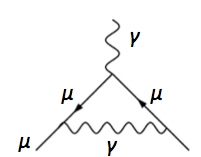
\includegraphics[scale=0.5]{figures/schwinger}
   \caption{The lowest-order (Schwinger) contribution to the muon magnetic moment anomaly.}
\label{label:schwinger}
\end{figure}

In fact, the QED calculation has been carried out to the fifth-loop contribution
\begin{equation}
a_{\mu}^{QED} = 116\,584\,718.951 \,\,\,\, (0.009)(0.019)(0.007)(0.077) \times 10^{-11}
\end{equation} 
with the uncertainties corresponding to the lepton mass ratios, the eight-order term in the four-loop contribution, the tenth-order term in the five-loop contribution, and the value of the fine structure constant $\alpha$ as provided by $^{87}$Rb atom where d$\alpha^{-1}\left(\text{Rb}\right) = 137.035\,999\,049(90)$ [0.066 ppb] \cite{alpha}.

\subsection{The Weak Contribution to $a_{\mu}$}

The weak contribution is the smallest correction to the anomaly that was first probed by E821.
The current electroweak calculation is performed up to two loops.
The leading electroweak effect originates from the single loop diagrams of W and Z bosons, as shown in Figure \ref{fig:weak} with a result of
\begin{equation}
a_{\mu}^{EW(1)} = 194.8 \times 10^{-11} 
\end{equation}
\begin{figure}
  \centering
  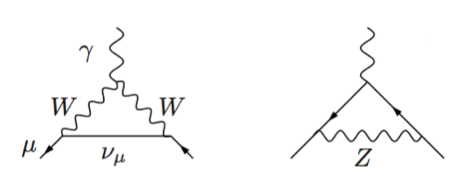
\includegraphics[scale=0.5]{figures/wz}
   \caption{Weak contributions to the muon anomalous magnetic moment with a one-loop diagrams with virtual W and Z gauge bosonss. }
  \label{fig:weak}
\end{figure}
The two-loop contribution is negative which reduces the weak contribution, and the third-loop contribution is negligible leading to a total result of 
\begin{equation}
a_{\mu}^{EW} = 153.6(1.0) \times 10^{-11} 
\end{equation}
where the error is due to unknown higher order contributions.
Since the weak contribution to the anomaly is of the order of 1.3 ppm, for this reason the current experimental precision of 0.54 ppm probes the weak scale of the SM. 

\subsection{Hadronic Contribution to $a_{\mu}$}

The hadronic contribution dominates the error in $a_{\mu}$ with an error of about 60 ppm. %?
This is due to the fact that the virtual hadrons that affect the anomaly have an energy scale of $m_{\mu}c^2$ which is below the QCD region that can be treated by perturbative methods. Alternatively, the hadronic 
It can be divided to three terms: the dominant lowest-order hadronic contribution and the hadronic light-by-light contribution, and the higher-order hadronic contribution.


\section{Beyond the Standard Model Implications}
\label{fut}

%% You need a file named `g-2_references.bib' to use BibTex here
\bibliography{g-2_references}


\appendix
\setcounter{chapter}{0}  % Try to change this!!
 \chapter{Spin Dynamics}
 \label{app:bmt}
 \chapter{Muon Decay Rate}
 \label{app:muon}
 \chapter{Radiative Corrections, Schwinger Term}

% \backmatter

% remarks:
% cyclotron period 149 ns
% muon-to-proton magnetic moment was determined as follow: measuremnt of the hyperfne interval of ground state muonium $\Delata \nu_{HFS}$ to 12 ppb. The theoritical prediction for the hyperfine inteval,  $\Delata \nu_{HFS,th}$ depends on $\mu_{\mu}/\mu_{\p}$, by equating the two, the ratio was determined to 30ppb. this value agrees with value a measurement of two zeeman hyperfine transtions in muonium in a strong magnetic field to 120 ppb. This means that the absolute calibration probe used to get the fre proton from the precession of the proton in water is good to 120ppb. See p51 BNL

\end{document}


